\begin{frame}
\frametitle{What is a Queue?}
\begin{columns}
  \column{0.3\textwidth}
    A queue is an example of a linear data structure, which works on the basis of "\textbf{first-in-first-out}" (FIFO).
  \column{0.55\textwidth}


  \tikzset{every picture/.style={line width=0.35pt}} %set default line width to 0.75pt

  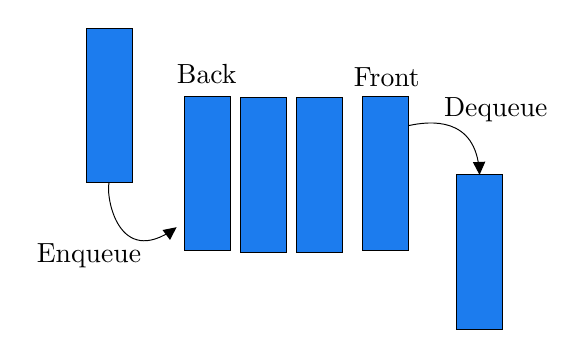
\begin{tikzpicture}[x=0.75pt,y=0.75pt,yscale=-0.70,xscale=0.70]
  %uncomment if require: \path (0,300); %set diagram left start at 0, and has height of 300

  \draw  [fill={rgb, 255:red, 28; green, 124; blue, 238 }  ,fill opacity=1 ]  (100, 62.67) rectangle (131.67, 169)   ;
  \draw  [fill={rgb, 255:red, 28; green, 124; blue, 238 }  ,fill opacity=1 ]  (138, 63.67) rectangle (169.67, 170)   ;
  \draw  [fill={rgb, 255:red, 28; green, 124; blue, 238 }  ,fill opacity=1 ]  (222, 62.67) rectangle (253.67, 169)   ;
  \draw  [fill={rgb, 255:red, 28; green, 124; blue, 238 }  ,fill opacity=1 ]  (177, 63.67) rectangle (208.67, 170)   ;
  \draw  [fill={rgb, 255:red, 28; green, 124; blue, 238 }  ,fill opacity=1 ]  (287, 116.67) rectangle (318.67, 223)   ;
  \draw  [fill={rgb, 255:red, 28; green, 124; blue, 238 }  ,fill opacity=1 ]  (32, 15.67) rectangle (63.67, 122)   ;
  \draw    (47.83,122) .. controls (45.36,131.57) and (54.15,181.65) .. (93.14,153.54) ;
  \draw [shift={(94.33,152.67)}, rotate = 503.13] [fill={rgb, 255:red, 0; green, 0; blue, 0 }  ][line width=0.75]  [draw opacity=0] (8.93,-4.29) -- (0,0) -- (8.93,4.29) -- cycle    ;

  \draw    (254.33,82.67) .. controls (268.12,79.71) and (300.35,75.79) .. (302.74,114.85) ;
  \draw [shift={(302.83,116.67)}, rotate = 267.9] [fill={rgb, 255:red, 0; green, 0; blue, 0 }  ][line width=0.75]  [draw opacity=0] (8.93,-4.29) -- (0,0) -- (8.93,4.29) -- cycle    ;


  \draw (34,172) node  [align=left] {Enqueue};
  \draw (314,72) node  [align=left] {Dequeue};
  \draw (115,47) node  [align=left] {Back};
  \draw (239,49) node  [align=left] {Front};


  \end{tikzpicture}

\end{columns}

\end{frame}


\begin{frame}
\frametitle{What is a Priority Queue?}

\begin{columns}
  \column{0.3\textwidth}
  A priority queue is like a regular queue or stack data structure but where additionally each element has a "\textbf{priority}" associated with it.
  In a priority queue, an element with high priority is served before an element with low priority.
  \column{0.5\textwidth}


  \tikzset{every picture/.style={line width=0.35pt}} %set default line width to 0.75pt

  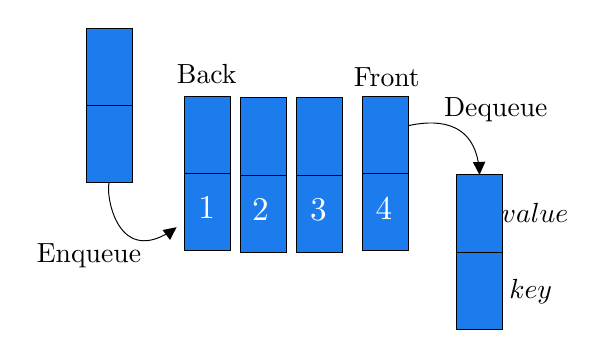
\begin{tikzpicture}[x=0.75pt,y=0.75pt,yscale=-0.70,xscale=0.70]
  %uncomment if require: \path (0,300); %set diagram left start at 0, and has height of 300

  \draw  [fill={rgb, 255:red, 28; green, 124; blue, 238 }  ,fill opacity=1 ]  (100, 62.67) rectangle (131.67, 169)   ;
  \draw  [fill={rgb, 255:red, 28; green, 124; blue, 238 }  ,fill opacity=1 ]  (138, 63.67) rectangle (169.67, 170)   ;
  \draw  [fill={rgb, 255:red, 28; green, 124; blue, 238 }  ,fill opacity=1 ]  (222, 62.67) rectangle (253.67, 169)   ;
  \draw  [fill={rgb, 255:red, 28; green, 124; blue, 238 }  ,fill opacity=1 ]  (177, 63.67) rectangle (208.67, 170)   ;
  \draw  [fill={rgb, 255:red, 28; green, 124; blue, 238 }  ,fill opacity=1 ]  (287, 116.67) rectangle (318.67, 223)   ;
  \draw  [fill={rgb, 255:red, 28; green, 124; blue, 238 }  ,fill opacity=1 ]  (32, 15.67) rectangle (63.67, 122)   ;
  \draw    (47.83,122) .. controls (45.36,131.57) and (54.15,181.65) .. (93.14,153.54) ;
  \draw [shift={(94.33,152.67)}, rotate = 503.13] [fill={rgb, 255:red, 0; green, 0; blue, 0 }  ][line width=0.75]  [draw opacity=0] (8.93,-4.29) -- (0,0) -- (8.93,4.29) -- cycle    ;

  \draw    (254.33,82.67) .. controls (268.12,79.71) and (300.35,75.79) .. (302.74,114.85) ;
  \draw [shift={(302.83,116.67)}, rotate = 267.9] [fill={rgb, 255:red, 0; green, 0; blue, 0 }  ][line width=0.75]  [draw opacity=0] (8.93,-4.29) -- (0,0) -- (8.93,4.29) -- cycle    ;

  \draw    (100,115.83) -- (131.67,115.83) ;
  \draw    (138,116.83) -- (169.67,116.83) ;
  \draw    (177,116.83) -- (208.67,116.83) ;
  \draw    (222,115.83) -- (253.67,115.83) ;
  \draw    (287,169.83) -- (318.67,169.83) ;
  \draw    (32,68.83) -- (63.67,68.83) ;

  \draw (237,140) node [scale=1.2]  {$\textcolor[rgb]{1,1,1}{4}$};
  \draw (192,141) node [scale=1.2]  {$\textcolor[rgb]{1,1,1}{3}$};
  \draw (152,141) node [scale=1.2]  {$\textcolor[rgb]{1,1,1}{2}$};
  \draw (115,139) node [scale=1.2]  {$\textcolor[rgb]{1,1,1}{1}$};

  \draw (338,197) node   {$key$};
  \draw (341,143) node   {$value$};

  \draw (34,172) node  [align=left] {Enqueue};
  \draw (314,72) node  [align=left] {Dequeue};
  \draw (115,47) node  [align=left] {Back};
  \draw (239,49) node  [align=left] {Front};


  \end{tikzpicture}

\end{columns}

\end{frame}
